\documentclass{article}

\usepackage[utf8]{inputenc}
\usepackage[T1]{fontenc}
\usepackage[norsk,english]{babel}   %norsk først så engelsk, så engelsk blir prioritert
\usepackage{graphicx}
\usepackage{amsmath}
\usepackage{listings}
\usepackage{multicol}
\usepackage[margin=2.54cm]{geometry}
\usepackage{wrapfig}

%Definerer hyperlinker og dens farger
\usepackage{hyperref}
\hypersetup{
    colorlinks,
    citecolor=blue,
    filecolor=black,
    linkcolor=blue,
    urlcolor=blue
}

%-----------------------------------

%Definerer farger til kodeeksemplene i PDF-en
\usepackage{color}

\definecolor{codegreen}{rgb}{0,0.6,0}
\definecolor{codegray}{rgb}{0.5,0.5,0.5}
\definecolor{codepurple}{rgb}{0.58,0,0.82}
\definecolor{backcolour}{rgb}{0.95,0.95,0.92}

\lstdefinestyle{mystyle}{
    backgroundcolor=\color{backcolour},
    commentstyle=\color{codegreen},
    keywordstyle=\color{magenta},
    numberstyle=\tiny\color{codegray},
    stringstyle=\color{codepurple},
    basicstyle=\footnotesize,
    breakatwhitespace=false,
    breaklines=true,
    captionpos=b,
    keepspaces=true,
    numbers=left,
    numbersep=5pt,
    showspaces=false,
    showstringspaces=false,
    showtabs=false,
    tabsize=2
}

\lstset{style=mystyle}

%------------------------------------

\setlength{\parindent}{0pt}
\setlength{\columnsep}{2mm} %column separation
\setlength{\columnsep}{10mm}

%\setlength{\arrayrulewidth}{1mm}
\setlength{\tabcolsep}{5mm}
\renewcommand{\arraystretch}{1.5}

\iffalse
If you want to change this temporarily, you can write:
\savegeometry{mydefaultgeometry}
\newgeometry{margin=3in}
And then later you can call:
\loadgeometry{mydefaultgeometry}
\fi

%for å fjerne overskriften "refrences" som kommer automatisk når man bruker bibtex
\usepackage{etoolbox}
\patchcmd{\thebibliography}{\section*{\refname}}{}{}{}

%----------------------------------------------------------------------------------------

\begin{document}

\addtocounter{page}{0}

\title{Project 3 \\
      \large For the course FYS3150}
\date{\today \\
    \vspace{1mm}
    \large Week 40 - ??}

\author{Erik Grammeltvedt, Erlend Tiberg North and Alexandra Jahr Kolstad}

\maketitle

%\newpage

%------------Her starter skrivingen-----------------------------------------

%\begin{multicols}{2}

\newpage
\clearpage

\textbf{Kommentarer fra project 1 på devilry:}

\begin{itemize}

\item Abstract: short motivation and presentation of the results and the findings \\

\item Introduction: you want to motive the reader about the problem and why you want solve it \\

\item Theory: explaining the theory behind the solution method and the problem \\

\item Method/implementation: how you implement the solution in order to fix/solve the problem \\

\item Results/graphs/tables: presenting the results \\

\item Discussion: Discussing the result from previous section \\

\item Conclusion: concluding the findings, your neutral opinion, etc… and future work \\

\item Appendix: How you derived your method, theory, etc… , altså utledning av ting i teori som ikke spesifikt er et bevis \\

\end{itemize}


Ting å gjøre for de ulike oppgavene:
\begin{itemize}

  \item 3a: beregne integralet, how many mesh points, lage et plott for å sjekke om grensene er passende å bruke \\

  \item 3b: finne grensene, erstatte Gauss-Legendre metoden med Laguerre polynomer, sammenligne med resultater fra a \\

  \item 3c: nå bruke brute force Monte Carlo, sammenligne resultatene med tidligere \\

  \item 3d: forbedre Monte Carlo med bruk av importance sampling, kommentere resultatene, lage en liste over tidene, sammenligne resultatene \\

  \item 3e: parallellisere koden fra 3d med openMP eller MPI, kommenter resultatene (hovedsakelig i tiden brukt)

\end{itemize}

\vspace{1cm}

\textbf{Det som mangler:}

\begin{itemize}
    \item må se gjennom abstract \\
    \item skrive mer på introduction \\
    \item lime inn theory \\
    \item skrive noe på method \\
    \item lime inn results \\
    \item skrive discussion \\
    \item skrive conclusion and perspective \\
    \item sjekke om vi skal ha noe i appendix \\
    \item sjekke references (den er skrevet dobbelt, er dette mulig å fjerne ? ) \\
\end{itemize}


%-------------------- Abstract -------------------------------
\vspace{1cm}


\begin{center}

{\Large\textbf{Abstract}} \label{sec:Abstract}

\end{center}

\vspace{5mm}

hensikt: tilnærme løsningen til integralet så best som mulig 5 pi**2 / 16**2 . \\

In this scientific study we will compute an integral with different numerical methods of integration to approximate the ground state correlation energy between two electrons in a helium atom. Our integral is given by equation (\ref{eq:integral}), which is not normalized. The integral has the analytical answer $\frac{5 \pi^2}{16^2} \approx 0.192765710958777$. The main interest and the goal of this study is to look at how the methods compare with different amount of mesh points and integration limits. The numerical integration methods we will use in this project are Gauss-Legendre quadrature, Gauss-Laguerre quadrature, brute force Monte Carlo, Monte Carlo with importance sampling, and Monte Carlo with parallization. The study was a success and proved Monte Carlo to be the fastest and most accurate method. Being based on big data, it required many more sampling points. However, as it did not manually calculate the integral, it was much more efficient. \\

SETT INN NOEN TALL SOM BEVIS HER

%All programs are found at our \href{https://github.com/Erikbgram/Fys3150}{GitHub-repository}. \\


\newpage

%------------------- Table of contents -----------------------

\vspace{1cm}

\tableofcontents

\vspace{1cm}

%-------------------- Introduction ------------------------------
\vspace{1cm}

\section{Introduction} \label{sec:Introduction}

The integral we are evaluating comes from the solution of Schrödinger's equation for a simplified case of determining the ground state correlation energy between two electrons in a helium atom.

\begin{equation} \label{eq:integral}
    \left\langle \frac{1}{| \vec{r_1} - \vec{r_2} |} \right\rangle = \int_{-\infty} ^\infty d \vec{r_1} d \vec{r_2} \hspace{1mm} e^{- 2 \alpha (r_1 + r_2)} \hspace{1mm} \frac{1}{| \vec{r_1} - \vec{r_2} |}
\end{equation}

The integral is not properly normalized. However, that is not important for the study.
If you are interested in how the integral is found, see \cite{task}.\\
Our aim is, as written in the abstract, to approximate this integral using two types of Gaussian Quadrature, and some variations of Monte Carlo. We have created a code that evaluates the integral using each method and compares them. Alongside the actual value we get the absolute value, and time used. Using this we present our data showing that Monte Carlo massively outperforms the other methods.\\
The report will go through the theory and methods behind our study and following that we will present our results and discuss them.

%-------------------- Theory ------------------------------------
\vspace{1cm}

\section{Theory} \label{sec:Theory}

\iffalse
  \begin{equation*} \label{eq:fullmatrixeq}
    \begin{bmatrix}
        d & a & 0 & \dots & 0 & 0 \\
        a & d & a & \dots & 0 & 0 \\
        0 & a & d & \dots & 0 & 0 \\
        \vdots & \vdots & \vdots & \ddots & \vdots & \vdots \\
        0 & 0 & 0 & a & d & a \\
        0 & 0 & 0 & 0 & a & d \\
    \end{bmatrix}
    \begin{bmatrix}
        u_1 \\
        u_2 \\
        u_3 \\
        \vdots \\
        u_{N-2} \\
        u_{N-1} \\
    \end{bmatrix}
      = \lambda
    \begin{bmatrix}
        u_1 \\
        u_2 \\
        u_3 \\
        \vdots \\
        u_{N-2} \\
        u_{N-1} \\
    \end{bmatrix}
  \end{equation*} \\
\fi
HER SKAL ERIK SITT INN\\
\\
\subsection{Theory of Gaussian Quadrature and the Gauss-Legendre- method}

The Gauss-Legendre method is based on the more general Gaussian Quadrature method witch uses Taylor series to solve an integral. The main idea is to generate weights, by solving sets of linear equations. For N pints in the Taylor series we get N weights. This weights are used in a weight function in order to approximate the integral.The theory behind Gaussian Quadrature is to obtain the weights by using orthogonal polynomials. This polynomials are orthogonal at certain intervals. For instance from [3,7] as an example. we can use these orthogonal polynomials in order to insure a smooth integral for are graph. The $x_i$ values are chosen arbitrary within the given interval. Together with the weights this gives us 2N parameters that can be used to solve the integral.
\newline
\newline

$I = \int_{a}^{b} f(x) = \int_{a}^{b}W(x)g(x)dx \approx  \sum_{n=1}^{N}  \omega_i g(x_i) $ (1)
\newline
\newline

In equation (1) we have the weight function W(x) and g(x) is a orthogonal polynomial that gives a smooths graph. Then we have the sum the weights, $\omega_i$, and the orthogonal polynomial $g(x_i)$ with a number of $x_i$ values within the given interval.
\newline
\newline

In order to go from Gaussian Quadrature to the Gauss-Legendre method a unit change is needed. Because the Gauss-Legendre method uses only the integral from [-1,1] and later apply the Gaussian Quadrature. A unit change is needed in order to use the Gauss-Legendre method.
\newline
\newline

Want to change t too $t = \frac{b-a}{2}x + \frac{a+b}{2}$
\newline
\newline

$\int_{a}^{b} f(t) dt = \frac{b-a}{2}\int_{-1}^{1} f(\frac{b-a}{2}x + \frac{a+b}{2}) dx$ (2)
\newline
\newline

Now exchanging this new integral, (2), into the Gaussian Quadrature, (1), the following estimate of the integral becomes,(3).
\newline
\newline

$\int_{a}^{b} f(t) dt \approx \frac{b-a}{2} \sum_{n=1}^{N} \omega_i f(\frac{b-a}{2}x + \frac{a+b}{2}) dx$ (3)


\subsection{Theory of the Montecarlo Method}




%--------------------- Method ------------------------------------
\vspace{1cm}

\section{Method} \label{sec:Method}

The methods used in this project are Gauss-Legendre quadrature, Gauss-Laguerre quadrature, brute force Monte Carlo, Monte Carlo with importance sampling, and Monte Carlo with parallization.

\subsection{Gauss-Legendre}

This method is excepted to give to worst approximation to the integral. This is because it uses approximations and other short cuts to more easily compute the integral. For instance the limits are originally given by $\pm \infty$ and in this method they have to be approximated to finite numbers.

integrand diverges.

THIS SHOULD ALSO BE ERIK SITT?

%--------------------- Results ----------------------------------
\vspace{1cm}

\section{Results} \label{sec:Results}

  \textit{Our results are as shown in the \nameref{sec:Appendix}}. We also have \texttt{.txt}-files for all the raw data generated by the projects up on \href{https://github.com/Erikbgram/Fys3150}{GitHub}. \\

\begin{itemize}

  \item How many mesh points do you need before the results converges at the level of the third leading digit?

  \item plottene for lambda, integrationspoints, montecarlo og timings

  \item tror ikke skal ha noen tabeller

\end{itemize}

  Burde ha at lambda er 2 siden det gir best resultater, se plottet fra plot\_data.txt.


  \begin{figure}[ht]
  	\centering
    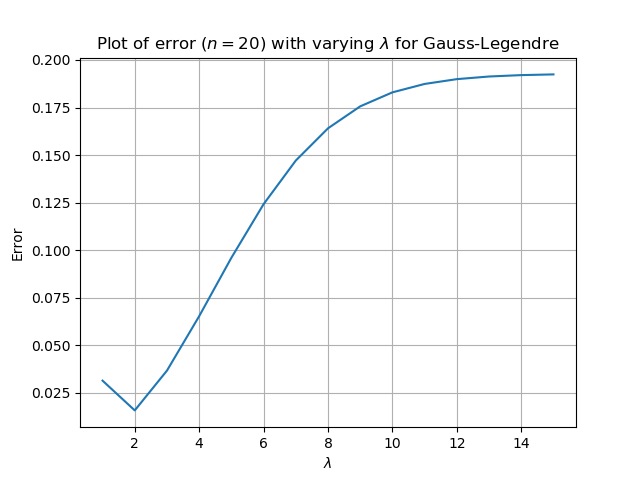
\includegraphics[width = 11cm]{images/error-lambda.png}
  	\caption{The plot of error as a function of lambda for Gauss-Legendre. }
    \label{fig:lambdapng}
  \end{figure}

  \begin{figure}[ht]
    \centering
    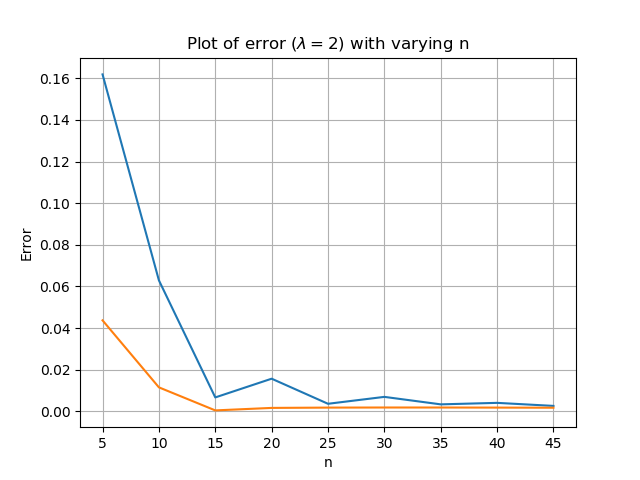
\includegraphics[width = 11cm]{images/error-integrationpoints.png}
    \caption{The plot of error as a function of integrations points $n$ for Gauss-Legendre and Gauss-Laguerre. }
    \label{fig:integrationpointspng}
  \end{figure}

    \begin{figure}[ht]
    \centering
    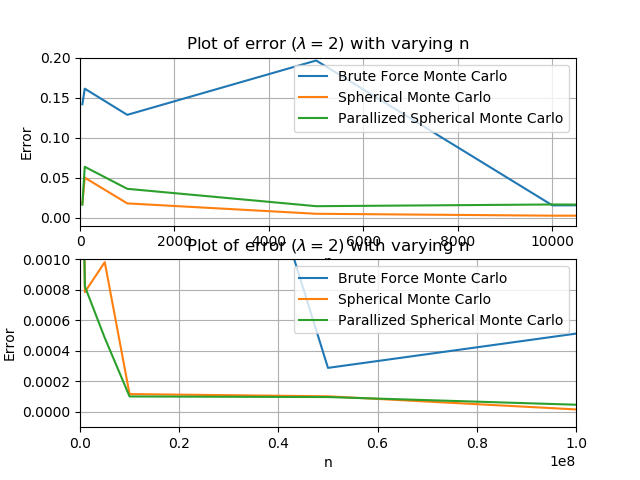
\includegraphics[width = 11cm]{images/error-montecarlo.png}
    \caption{The plot of error as a function of integration points $n$ for brute force Monte Carlo, spherical Monte Carlo with importance sampling, and parallized spherical Monte Carlo with importance sampling. }
    \label{fig:montecarlopng}
  \end{figure}

%\vspace{3cm}



  \begin{table}[ht] \label{tab:error-Gauss}
    \centering
      \caption{Error and execution time for Gauss-Legendre and Gauss-Laguerre.}
      \vspace{2mm}
      \begin{tabular}{|c|c|c|c|}
        \hline
        Legendre error & Laguerre error & Legendre time & Laguerre time   \\
        \hline \hline
        0.161836 & 0.0437248 & 0.00082727 & 0.0022169 \\
        0.0629315 & 0.0115411 & 0.0520311 & 0.150486 \\
        0.00670907 & 0.000476827 & 0.609131 & 1.69456 \\
        0.0157005 & 0.00167232 & 3.35013 & 9.3416 \\
        0.00365618 & 0.00181852 & 12.8663 & 35.5266 \\
        0.00697009 & 0.00186703 & 38.0615 & 105.708 \\
        0.00337855 & 0.00186074 & 95.5971 & 264.104 \\
        0.00409558 & 0.00181934 & 214.105 & 608.182 \\
        0.00263748 & 0.00176034 & 433.725 & 1191.8 \\
        0.00281127 & 0.00169433 & 831.449 & 2314.1 \\
        \hline
      \end{tabular} \\
      \hspace{0pt}\\
  \end{table}

    \begin{table}[ht] \label{tab:error-MonteCarlo}
    \centering
      \caption{Error and execution time for Gauss-Legendre and Gauss-Laguerre.}
      \vspace{2mm}
      \begin{tabular}{|c|c|c|c|c|c|}
        \hline
        BMC error & SMC error & PSMC error & BMC time & SMC time & PSMC time  \\
        \hline \hline
        0.138417 & 0.251552 & 0.131809 & 0.00011814 & 8.7853e-05 & 0.00038 \\
        0.157825 & 0.156198 & 0.0071997 & 0.00014777 & 0.0001193 & 0.00037 \\
        0.113224 & 0.012164 & 0.00302251 & 0.0003764 & 0.0003822 & 0.00051 \\
        0.079204 & 0.0168798 & 0.022215 & 0.00066215 & 0.0007048 & 0.00098 \\
        0.029304 & 0.011712 & 0.013536 & 0.0029481 & 0.00338986 & 0.002612 \\
        0.0457817 & 0.00027297 & 0.018113 & 0.005808 & 0.006558 & 0.005258 \\
        0.0096648 & 0.0038374 & 0.0012646 & 0.029013 & 0.032508 & 0.025366 \\
        0.024003 & 0.0043587 & 0.00030587 & 0.056982 & 0.067961 & 0.047938 \\
        0.0137398 & 0.0046188 & 0.00356363 & 0.287352 & 0.328019 & 0.18964 \\
        0.0161491 & 0.00049579 & 0.0005530 & 0.57400 & 0.654257 & 0.354581 \\
        0.00311977 & 0.00048176 & 0.00026134 & 2.85616 & 3.27695 & 1.82245 \\
        0.00481115 & 0.00012881 & 2.40583e-05 & 5.70269 & 6.54182 & 3.3623 \\
        0.00265522 & 9.08138e-05 & 5.988e-05 & 29.7091 & 33.0613 & 16.5097 \\
        0.00117823 & 0.0001726 & 7.16594e-05 & 58.8054 & 67.2903 & 33.4236 \\
        6.0793e-05 & 2.5923e-05 & 1.6625e-05 & 415.953 & 448.229 & 208.211 \\
        \hline
      \end{tabular} \\
      \hspace{0pt}\\
  \end{table}




%--------------- Discussion ---------------------------------------
\vspace{1cm}

\section{Discussion} \label{sec:Discussion}

diskutere resultatetene: altså hvilke metoder som brukte lengst tid, hvilke som var mest nøyaktig osv \\
koble dette til teori for hvorfor resultatene ble slik som de er \\
\\
The results show that the parallized code actually isn't better than the non-parallized code. This is strang. However, it can be from the fact that the computer running the code only has two cores so there is less of an effect.

%---------------Conclusion and perspective---------------------------
\vspace{1cm}

\section{Conclusion and perspective} \label{sec:Conclusion}

To conclude the Monte Carlo integration methods exceeded the Gauss quadrature methods for both computation time and accuracy of the answer to the integral. As expected the parallized spherical Monte Carlo with importance sampling is the fastest method with the highest degree of accuracy. This is mainly because ... \\

legge inn mer her som knytter det opp til teorien.


%--------------Appendix---------------------------------------------
\vspace{1cm}

\section{Appendix} \label{sec:Appendix}

Figure (\ref{fig:timingslargepng}) does not include all larger data points from our \texttt{.txt}-files. These can be found in table (???????)

\begin{figure}[ht]
\centering
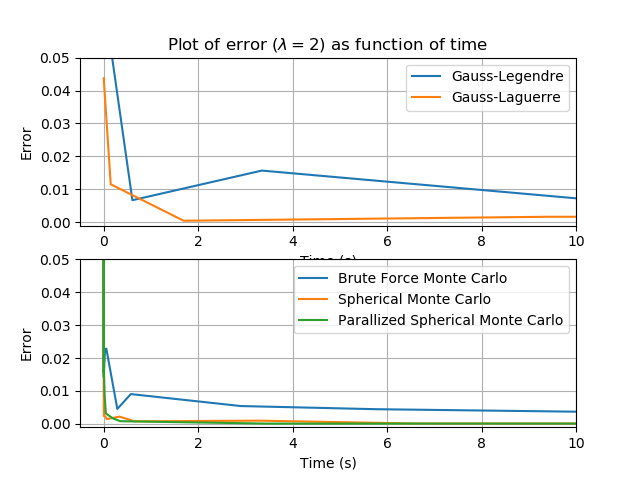
\includegraphics[width = 11cm]{images/method-timings-small.png}
\caption{The plot of error as a function of time for all the numerical integration methods used in this scientific study. }
\label{fig:timingssmallpng}
\end{figure}

\begin{figure}[ht]
\centering
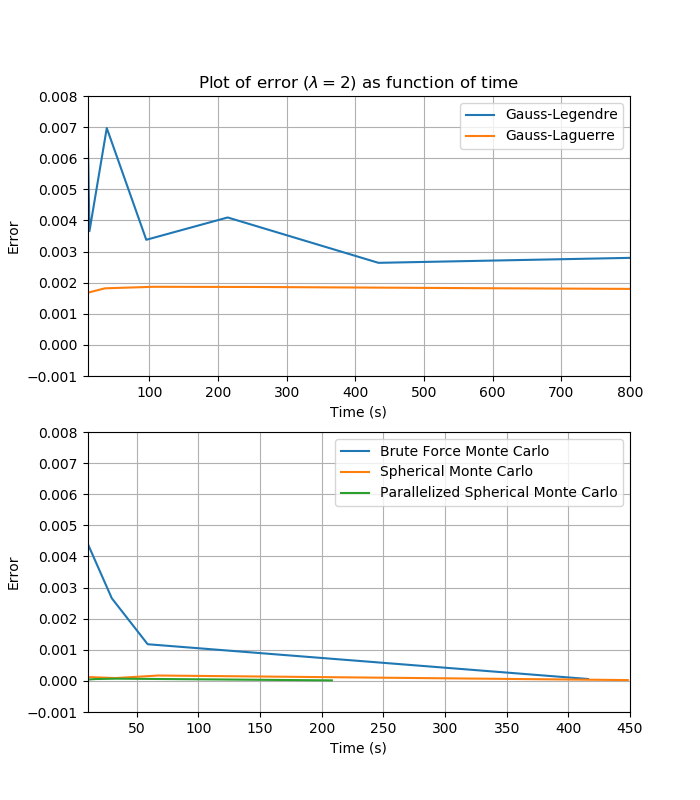
\includegraphics[width = 11cm]{images/method-timings-large.png}
\caption{This figure is a continuation of the previous figure, (\ref{fig:timingssmallpng}). }
\label{fig:timingslargepng}
\end{figure}


%\clearpage

%----------------References----------------------------------------
\vspace{1cm}

\section{References} \label{sec:References}

\begin{thebibliography}{}

\bibitem{task}
Morten H. Jensen (2019), \href{https://github.com/CompPhysics/ComputationalPhysics/blob/master/doc/Projects/2019/Project3/pdf/Project3.pdf}{Project 3}, Departement of Physics, University of Oslo, Norway

\bibitem{github}
Erik B. Grammeltvedt, Alexandra Jahr Kolstad, Erlend T. North (2019), \href{https://github.com/Erikbgram/Fys3150}{GitHub}, Students of Departement of Physics, University of Oslo, Norway

\bibitem{lecture_slides}
Morten H. Jensen (2015), \href{https://github.com/CompPhysics/ComputationalPhysics/blob/master/doc/Lectures/lectures2015.pdf}{Lecture slides for FYS3150}, Department of Physics, University of Oslo, Norway

\end{thebibliography}


%----------------Slutten av dokumentet---------------------------------------


%\end{multicols}

\end{document}
